\chapter{State of the Art}

\section{Multi-View Geometry}
\subsection{Structure-from-Motion}
Structure-from-Motion (SfM) jointly estimates camera poses and sparse scene geometry from multiple images \cite{hartley2004multiple}. In this thesis, SfM is performed with COLMAP \cite{schoenberger2016sfm,schoenberger2016mvs}.
\begin{figure}[H]
    \centering
    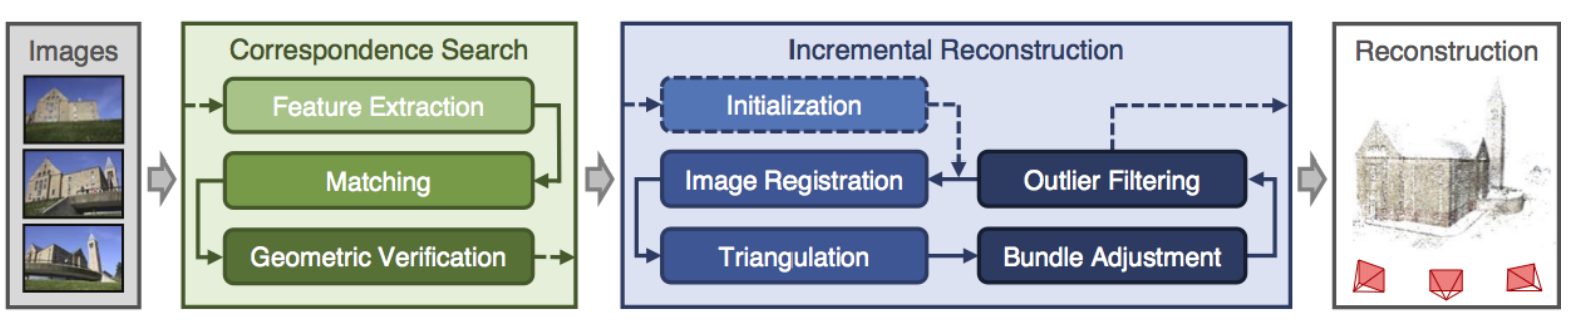
\includegraphics[width=0.8\textwidth]{images/COLMPA_pipeline.png}
    \caption{End-to-end SfM pipeline: feature extraction and matching, geometric verification, incremental camera/point estimation, and bundle adjustment.}
    \label{fig:sfm_pipeline_overview}
\end{figure}
SfM aims to recover both the 3D structure of a scene and the camera parameters that explain a set of images acquired from different viewpoints. In incremental pipelines such as COLMAP, this process is typically organized into the following stages:
\begin{enumerate}
    \item keypoint extraction;
    \item keypoint matching and geometric verification;
    \item incremental pose and sparse structure estimation;
    \item bundle adjustment refinement.
\end{enumerate}
The following exposition follows roughly this pipeline, from local features through two-view geometry, pose and triangulation, and finally bundle adjustment, with emphasis on geometric quantities that later become inputs to neural rendering methods.

\paragraph{Keypoint extraction (SIFT).}
The SfM pipeline starts from local visual evidence, and COLMAP commonly uses SIFT features \cite{lowe2004sift}. The scale-space representation is
\[
L(x,y,\sigma)=G(x,y,\sigma)\ast I(x,y),
\]
and keypoint candidates are selected as extrema of the Difference of Gaussians:
\[
D(x,y,\sigma)=L(x,y,k\sigma)-L(x,y,\sigma).
\]
SIFT then performs keypoint localization, orientation assignment, and descriptor computation. Each descriptor is a 128-dimensional vector.

\begin{figure}[H]
    \centering
    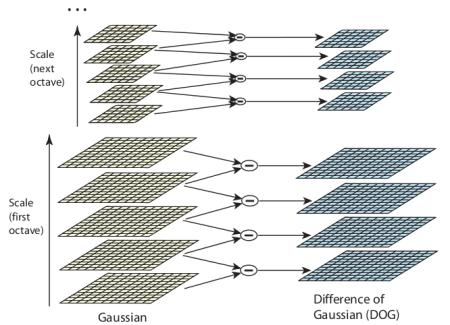
\includegraphics[width=0.5\textwidth]{images/sift_dog.jpg}
    \caption{Difference-of-Gaussians (DoG) used for scale-space extrema detection in SIFT.}
    \label{fig:sift_dog}
\end{figure}

The SIFT pipeline can be summarized in four steps:
\begin{itemize}
    \item \textbf{Scale-space extrema detection:} build $L$ and detect extrema of $D$.
    \item \textbf{Keypoint localization:} reject low-contrast candidates and unstable edge responses.
    \item \textbf{Orientation assignment:} estimate a dominant orientation from local gradients to achieve rotation invariance.
    \item \textbf{Descriptor computation:} aggregate gradient orientation histograms into a descriptor $d\in\mathbb{R}^{128}$.
\end{itemize}


These descriptors are designed to be robust to moderate illumination changes, scale changes, and rotations.

\paragraph{Descriptor matching.}
Once descriptors are extracted, the next step is to establish correspondences across views. Given images $I$ and $J$ with descriptor sets
\[
\mathcal{D}_I = \{d_I^1, \dots, d_I^{n_I}\}, \qquad
\mathcal{D}_J = \{d_J^1, \dots, d_J^{n_J}\},
\]
\begin{figure}[H]
    \centering
    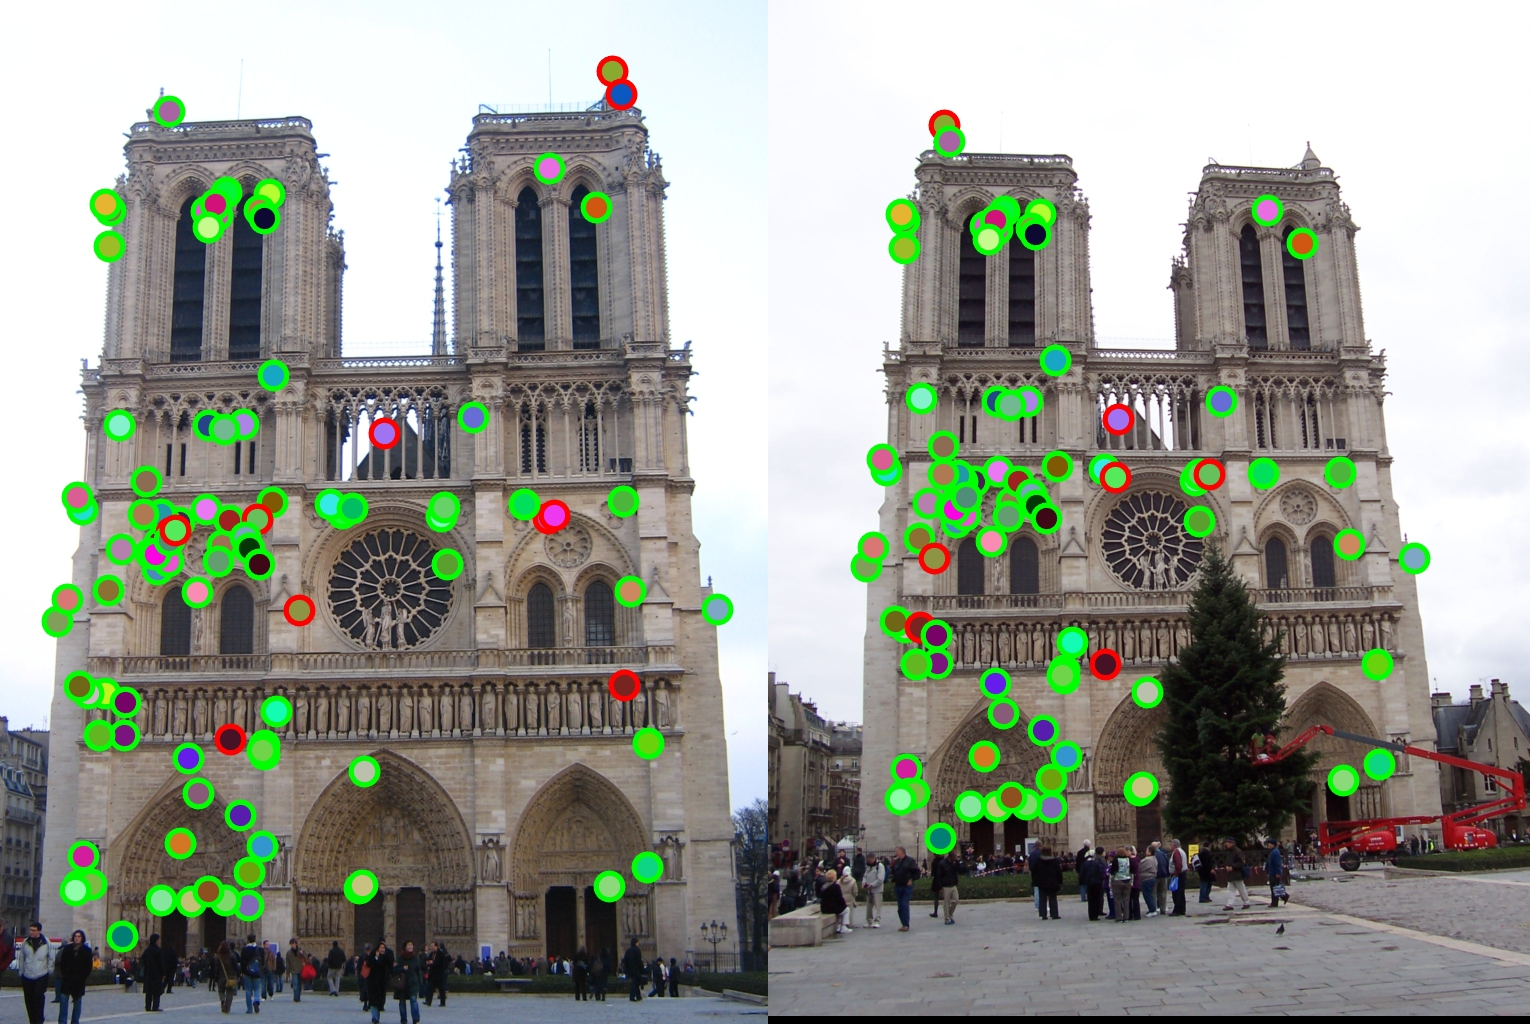
\includegraphics[width=0.3\textwidth]{images/keypoints_sift.jpg}
    \caption{SIFT keypoints detected over an image, before geometric matching across views.}
    \label{fig:sift_keypoints_only}
\end{figure}
matching is based on nearest-neighbor distance:
\[
\operatorname{dist}(d_i,d_j)=\|d_i-d_j\|_2.
\]
In practice, approximate nearest-neighbor search and Lowe's ratio test are applied for efficiency and robustness.

For a descriptor $d_I^m$ in image $I$, a nearest neighbor in image $J$ can be written as
\[
j^\star(m)=\arg\min_{p\in\{1,\dots,n_J\}} \left\|d_I^m-d_J^p\right\|_2.
\]
If the dataset contains $N$ images, naive exhaustive matching considers $\binom{N}{2}$ image pairs, which becomes expensive as $N$ grows. For this reason, practical systems restrict candidate pairs using scene overlap heuristics and accelerate nearest-neighbor search with libraries such as FLANN.

\begin{figure}[H]
    \centering
    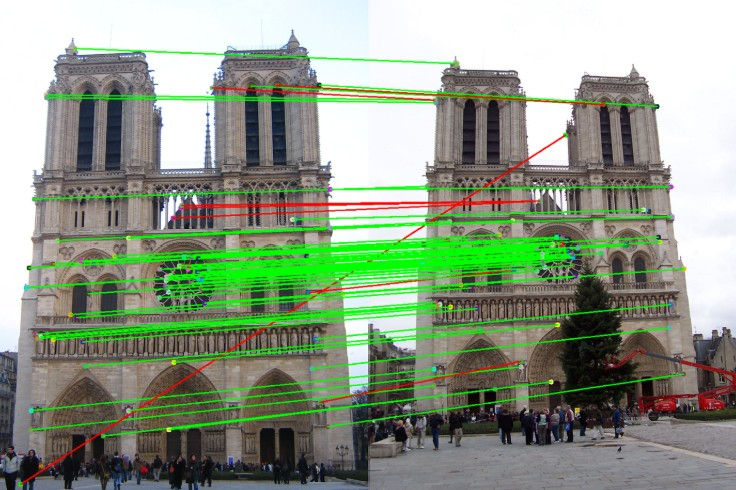
\includegraphics[width=0.3\textwidth]{images/matching_keypoints_SIFT.jpg}
    \caption{Example of SIFT keypoint correspondences between two views used for geometric verification and triangulation.}
    \label{fig:sift_keypoint_matching}
\end{figure}

\paragraph{Camera model and projection.}
After correspondences are defined in image space, camera projection links them to 3D geometry. A homogeneous 3D point $X=(X,Y,Z,1)^\top$ is projected to image point $x=(u,v,1)^\top$ via
\[
x \sim PX, \qquad P = K[R\mid t],
\]
with intrinsic matrix
\[
K=
\begin{bmatrix}
f_x & s & c_x \\
0 & f_y & c_y \\
0 & 0 & 1
\end{bmatrix}.
\]

\paragraph{SfM reconstruction and the observation graph.}
With this projection model in place, SfM estimates intrinsic parameters $K$, extrinsic parameters $(R,t)$ for each image, and a sparse set of 3D points $\{X_j\}$. 3D points are obtained by triangulation from multi-view correspondences. During incremental reconstruction, COLMAP maintains an \emph{observation graph} that links each 3D point to the images where it is observed. This graph is central for bundle adjustment because it defines which reprojection residuals are active for each parameter block.

In many COLMAP setups, all images from the same camera share a single intrinsic calibration $K$, while each image has its own pose $(R,t)$.

\paragraph{Epipolar geometry.}
Building on the previous matching and projection steps, epipolar geometry provides the key geometric link between image correspondences and relative camera pose: for corresponding points $x_1$ and $x_2$ in two views, the epipolar constraint is
\[
x_2^\top F x_1 = 0,
\]
where $F$ is the fundamental matrix (rank 2). With known intrinsics, the essential matrix is
\[
E = K^\top F K = [t]_\times R,
\]
with
\[
[t]_\times=
\begin{bmatrix}
0 & -t_z & t_y \\
t_z & 0 & -t_x \\
-t_y & t_x & 0
\end{bmatrix}.
\]

\begin{figure}[H]
    \centering
    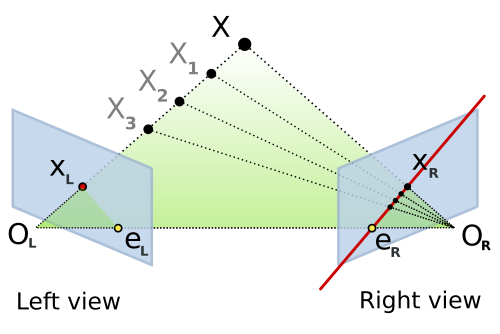
\includegraphics[width=0.3\textwidth]{images/Epipolar_geometry.svg.png}
    \caption{Two-view epipolar geometry with baseline, epipoles, and epipolar lines satisfying $x_2^\top F x_1=0$.}
    \label{fig:epipolar_geometry}
\end{figure}

The physically valid pose is selected with the cheirality condition after triangulation: the reconstructed points must be in front of the cameras.

Geometrically, epipolar geometry constrains correspondences: if $x_1$ is known in the first image, the match in the second image must lie on the epipolar line. In homogeneous coordinates, the epipolar line in the second image can be written as $l_2 \sim F x_1$. The epipole is the intersection of all epipolar lines in an image and corresponds to projecting the other camera center into the image plane.

\paragraph{Essential matrix (calibrated two-view geometry).}
To move from general two-view constraints to calibrated geometry, it is convenient to work in normalized image coordinates when intrinsic parameters are known:
\[
\hat{x} = K^{-1}x.
\]
In normalized coordinates, the epipolar constraint is expressed by the essential matrix $E$ as
\[
\hat{x}_2^\top E \hat{x}_1 = 0,
\qquad
E=[t]_\times R.
\]
The essential matrix has five degrees of freedom and, in the noise-free case, its singular values satisfy the characteristic constraint of a normalized essential matrix (two equal nonzero singular values and one zero singular value). With noisy measurements, a standard correction is to compute the SVD $E=U\Sigma V^\top$ and replace $\Sigma$ by a rank-2 matrix that enforces the essential-matrix singular-value pattern.

From $E$, one can recover up to four candidate motions $(R,t)$. The physically consistent solution is selected using cheirality after triangulating a set of points: the correct candidate maximizes the number of points with positive depth in both cameras.

\paragraph{Fundamental matrix estimation.}
Complementarily, for uncalibrated settings one works with the fundamental matrix, which encodes two-view geometry and has rank $2$. With at least eight point correspondences, one can formulate a linear system $Af=0$ where $f$ is a vectorization of $F$ and $A$ is built from the constraints $x_2^\top F x_1=0$. The minimal solution is obtained from the singular vector associated with the smallest singular value of $A$. Because noise breaks the rank constraint, a common post-processing step is to compute the SVD of the estimated matrix and set the smallest singular value to zero.

In practice, $F$ is commonly estimated with robust procedures such as the normalized 8-point algorithm embedded in RANSAC \cite{fischler1981ransac}. The linear system is solved up to scale and then projected to rank 2 by SVD. This step is essential because outlier correspondences from repeated textures, specularities, or dynamic objects can otherwise corrupt camera pose estimation.

\subsection{Camera Pose Estimation}
Building on these constraints, camera pose can be recovered from essential-matrix decomposition in calibrated two-view settings, or from Perspective-$n$-Point (PnP) when 2D--3D correspondences are available.

PnP is usually formulated as
\[
\min_{R,t} \sum_{k=1}^{n}\left\|\pi\!\left(K(RX_k+t)\right)-u_k\right\|_2^2.
\]
Incremental SfM typically alternates pose estimation, triangulation of new points, and local/global BA refinement.

From a geometric standpoint, two-view calibrated pose estimation from $E$ yields four candidate $(R,t)$ solutions. The correct one is chosen by enforcing positive depth (cheirality) for triangulated points in both cameras. This constraint is a key consistency check and removes physically invalid configurations.

\paragraph{PnP algorithms.}
Several specialized solvers exist for PnP, including minimal solvers (e.g., P3P) and efficient $n$-point formulations (e.g., EPnP). In incremental SfM, PnP is commonly used to register a new image once a sufficient set of 3D--2D correspondences is available from previously reconstructed structure.

\subsection{Sparse 3D Reconstruction}
Once camera poses are estimated, triangulation turns calibrated correspondences into 3D point coordinates. A linear estimate is usually computed first and then refined by nonlinear reprojection-error minimization.

\paragraph{Triangulation objective.}
For point observations across views, a common formulation is
\[
\min_{\tilde{X}} \sum_{j=1}^{M} \left\| \tilde{x}_j-\pi(P_j\tilde{X}) \right\|_2^2,
\]
where $\tilde{x}_j$ are measured image points, $P_j$ are known projection matrices for $M$ views, and $\tilde{X}$ is the unknown homogeneous 3D point.
This optimization is nonlinear due to perspective division; therefore, iterative solvers are used after linear initialization.

\paragraph{Linear initialization.}
A standard approach is the Direct Linear Transform (DLT) formulation, which rewrites each correspondence as linear constraints on $\tilde{X}$ and solves for $\tilde{X}$ in homogeneous coordinates up to scale. The linear estimate is subsequently refined by Gauss--Newton or Levenberg--Marquardt minimization of reprojection error.

When the baseline between views is too small, triangulation becomes ill-conditioned and depth uncertainty increases. For this reason, view selection and track quality have direct impact on reconstruction stability.

\paragraph{Bundle adjustment.}
After estimating camera poses and triangulating a sparse point cloud (possibly over several incremental steps), pipelines such as COLMAP tighten global consistency by minimizing reprojection error over all cameras and jointly over all tied 3D parameters. Let $\{C_i\}$ be camera parameters, $\{X_j\}$ 3D points, and $V_{ij}$ visibility. Bundle adjustment solves
\[
\min_{\{C_i\},\{X_j\}}
\sum_{i=1}^{I}\sum_{j=1}^{J}V_{ij}\,
\left\|
\pi(C_i, X_j)-x_{ij}
\right\|_2^2,
\]
where $\pi$ is projection into the image plane.

Bundle adjustment is a large sparse nonlinear least-squares problem. Modern SfM systems exploit the block-sparse structure of Jacobians and the Schur complement to optimize efficiently. This refinement is often the main factor behind the final metric quality of camera trajectories and sparse structure.

Bundle adjustment is a large sparse nonlinear least-squares problem. Modern SfM systems exploit the block-sparse structure of Jacobians and the Schur complement to optimize efficiently; implementations typically use sparse solvers (e.g.\ Ceres Solver) tailored to the sparsity pattern induced by the visibility structure. This refinement is often the main factor behind the final metric quality of camera trajectories and sparse structure.


\section{Neural Scene Representations}
\subsection{Neural Radiance Fields}
Having established the multi-view geometric background, we can now transition to neural scene representations. Before introducing NeRF, it is useful to recall the plenoptic function
\[
P(x,y,z,\theta,\phi,\lambda,t),
\]
which describes the intensity of light passing through a point in space along a direction, as a function of wavelength and time. A radiance field can be viewed as a simplified instance of this description, tailored to static scene reconstruction and rendering.

More formally, a radiance field maps position and viewing direction to emitted color and volume density:
\[
F(\mathbf{x},\mathbf{d}) \rightarrow (\mathbf{c},\sigma),
\]
where $\mathbf{x}\in\mathbb{R}^3$, $\mathbf{d}$ is a unit viewing direction, $\mathbf{c}$ is RGB color, and $\sigma$ is a nonnegative density that controls occlusion and transparency along rays.

Two broad families are commonly used to represent radiance fields:
\begin{enumerate}
    \item \textbf{Implicit representations}, where $F$ is implemented by a neural network, as in NeRF \cite{mildenhall2020nerf}.
    \item \textbf{Explicit representations}, where $F$ is stored using discrete structures such as voxel grids, point clouds, or collections of parametric primitives (including Gaussian-based methods).
\end{enumerate}

\paragraph{Neural Radiance Fields (NeRF).}
Starting from this formulation, NeRF \cite{mildenhall2020nerf} approximates the radiance field with an MLP $F_\Theta$:
\[
F_\Theta(\mathbf{x},\mathbf{d}) \rightarrow (\mathbf{c},\sigma),
\]
where $\Theta$ denotes learnable parameters. The scene geometry and appearance are therefore encoded implicitly in network weights rather than in an explicit mesh.

\begin{figure}[H]
    \centering
    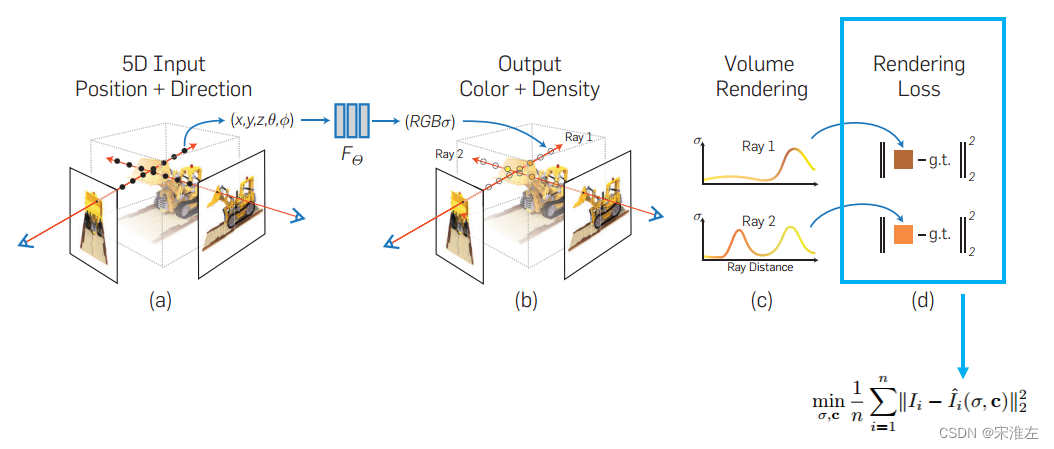
\includegraphics[width=0.8\textwidth]{images/NeRF.png}
    \caption{NeRF ray-based rendering: sample evaluation along rays and volumetric compositing of color and density.}
    \label{fig:nerf_ray_rendering}
\end{figure}

\paragraph{Ray casting and volume rendering.}
To connect the representation to image synthesis, NeRF renders by casting one ray per pixel from a given camera. A ray is parameterized by
\[
\mathbf{r}(t)=\mathbf{o}+t\mathbf{d},
\]
where $\mathbf{o}$ is the camera center and $\mathbf{d}$ is the ray direction.

NeRF does not intersect rays with explicit surfaces. Instead, it performs ray marching by sampling points $\{\mathbf{r}(t_i)\}_{i=1}^{N}$ between near and far bounds $(t_n,t_f)$. At each sample, the network predicts a color $\mathbf{c}_i$ and density $\sigma_i$. The predicted pixel color is obtained by the volume rendering integral
\[
C(\mathbf{r})=\int_{t_n}^{t_f} T(t)\,\sigma(\mathbf{r}(t))\,\mathbf{c}(\mathbf{r}(t),\mathbf{d})\,dt,
\]
with transmittance
\[
T(t)=\exp\!\left(-\int_{t_n}^{t}\sigma(\mathbf{r}(s))\,ds\right).
\]

\paragraph{Discrete approximation.}
For implementation, the continuous integral is approximated by a finite sum over ordered samples along the ray:
\[
\hat{C}(\mathbf{r})=\sum_{i=1}^{N}T_i\,\alpha_i\,\mathbf{c}_i,\quad
\alpha_i=1-\exp(-\sigma_i\delta_i),\quad
T_i=\prod_{j=1}^{i-1}(1-\alpha_j),
\]
where $\delta_i$ is the distance between consecutive samples. The term $\alpha_i$ can be interpreted as the probability that the ray terminates at sample $i$, while $T_i$ is the probability that the ray reaches sample $i$ without being absorbed earlier. This construction naturally models occlusion, semi-transparency, and view-dependent appearance when $\mathbf{c}_i$ depends on $\mathbf{d}$.

\paragraph{Training procedure.}
Given this rendering formulation, NeRF is trained from a set of images with known camera poses. For each sampled ray, the model renders $\hat{C}(\mathbf{r})$ and compares it to the ground-truth color $C_{\text{gt}}(\mathbf{r})$. A typical objective is mean squared error:
\[
\mathcal{L} = \sum_{\mathbf{r}}\left\|\hat{C}(\mathbf{r})-C_{\text{gt}}(\mathbf{r})\right\|_2^2.
\]


\subsection{3D Gaussian Splatting}
3D Gaussian Splatting (3DGS) represents a scene with explicit anisotropic Gaussian primitives optimized from calibrated views \cite{kerbl2023gaussian}. It combines high-quality rendering with real-time rasterization and builds on splatting principles connected to surface and EWA volume splatting \cite{zwicker2001surface,zwicker2002ewa}.

Similarly to NeRF, the goal is to reconstruct scene appearance from calibrated images and render novel viewpoints. However, the representation is fundamentally different: NeRF stores the radiance field implicitly in network weights, while 3DGS stores it explicitly as a collection of learnable volumetric primitives. Each Gaussian is defined by a position, an anisotropic shape, an opacity, and appearance parameters. In this sense, 3DGS still models density, color, visibility, and viewpoint, but without per-ray MLP queries.

This distinction matters for geometry: although optimized Gaussians often align with visible surfaces, they do not define a closed boundary mesh. Several primitives can overlap along the same viewing ray and still reduce photometric error without agreeing on a single depth, so the representation remains volumetric rather than a unique surface per object. 3DGS is therefore particularly strong for photorealistic novel view synthesis, while explicit geometry extraction remains challenging.

Compared to NeRF, 3DGS removes per-sample MLP evaluation along rays and instead projects explicit primitives directly to screen space. This architectural shift is central for real-time performance while preserving high rendering fidelity.

\begin{figure}[H]
    \centering
    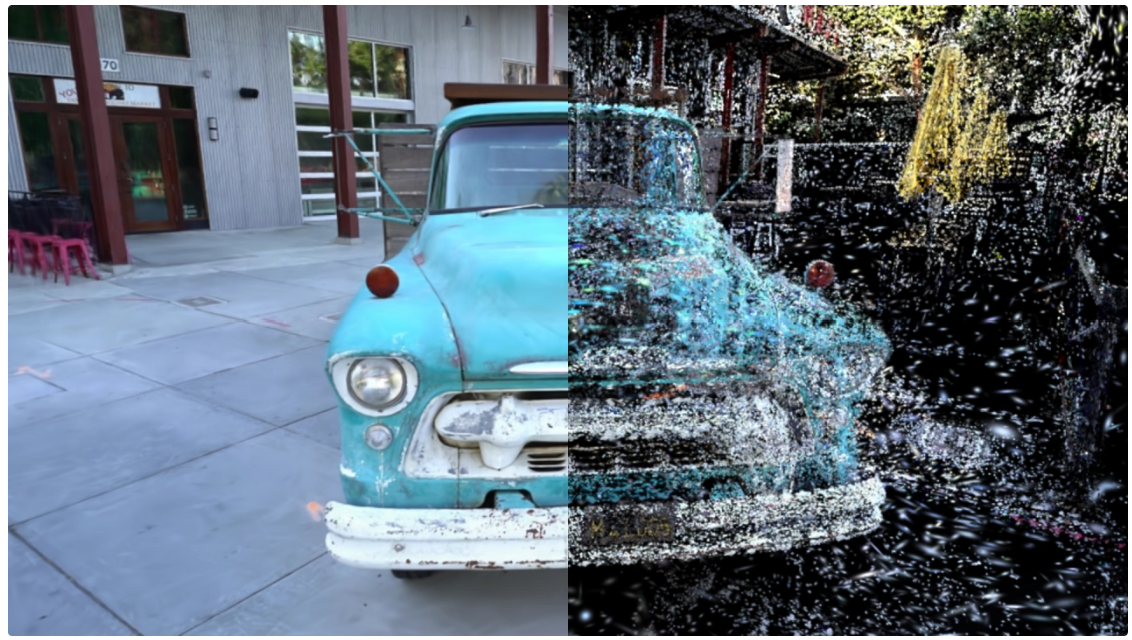
\includegraphics[width=0.5\textwidth]{images/result_3d_gaussian.png}
    \caption{Representative qualitative reconstruction/rendering result obtained with 3D Gaussian Splatting.}
    \label{fig:nerf_vs_3dgs}
\end{figure}

\subsubsection{Pipeline overview}
The full 3DGS pipeline can be summarized as:
\begin{enumerate}
    \item SfM-based data processing (camera calibration and sparse points);
    \item Gaussian initialization from sparse geometry;
    \item splatting-based rendering and alpha compositing;
    \item differentiable optimization of Gaussian parameters;
    \item adaptive density control (clone, split, prune);
    \item tile-based rasterization for efficient screen-space processing.
\end{enumerate}

\begin{figure}[H]
    \centering
    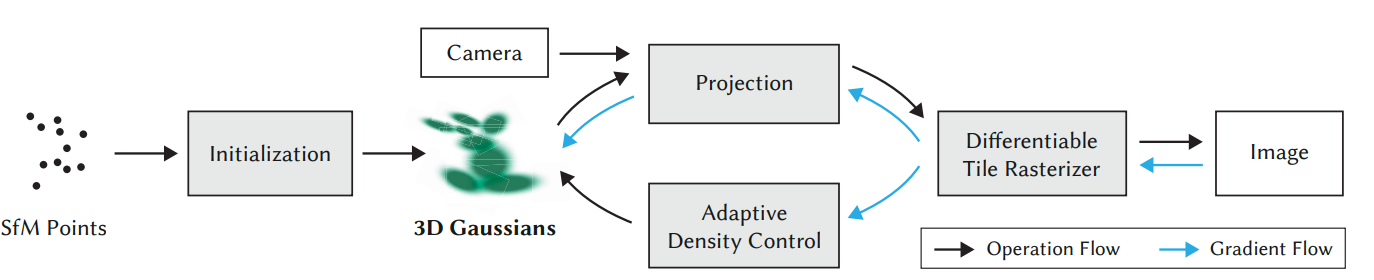
\includegraphics[width=0.7\textwidth]{images/full3dgaussiansplattinn.png}
    \caption{3DGS pipeline: SfM-based data processing, Gaussian initialization, splatting-based rendering and alpha compositing, differentiable optimization of Gaussian parameters, adaptive density control (clone, split, prune), tile-based rasterization for efficient screen-space processing.}
    \label{fig:3dgs_pipeline}
\end{figure}

\subsubsection{Relation with previous splatting methods}
Before detailing 3DGS, it is useful to recall the general idea of \emph{splatting}. In splatting, discrete primitives are projected to the image plane and accumulated into a continuous image. Each primitive defines a footprint in screen space and contributes to all pixels inside that footprint with weights given by a reconstruction kernel.

This is a forward-rendering viewpoint:
\begin{itemize}
    \item define primitives in world/object space;
    \item project them to screen space;
    \item compute a footprint region;
    \item accumulate weighted contributions into the framebuffer.
\end{itemize}
This differs from NeRF-style ray marching, where each pixel ray is traced independently through the volume.

\paragraph{Surface splatting.}
Surface splatting \cite{zwicker2001surface} renders surfaces represented by point samples without requiring an explicit triangle mesh. Each point is associated with a local surface element (\emph{surfel}) that projects to an elliptical footprint. From a signal-processing perspective, the rendered image can be understood as a weighted reconstruction of point attributes:
\[
f(\mathbf{x})=\sum_k w_k(\mathbf{x})\,f_k,
\]
where $f_k$ is an attribute (e.g., color) at sample $k$ and $w_k(\mathbf{x})$ depends on the distance between the pixel $\mathbf{x}$ and the projected footprint.

A central idea is Elliptical Weighted Average (EWA) filtering, which adapts the reconstruction kernel to anisotropic footprints induced by perspective projection. This reduces aliasing by combining reconstruction with a screen-space prefilter.

\begin{figure}[H]
    \centering
    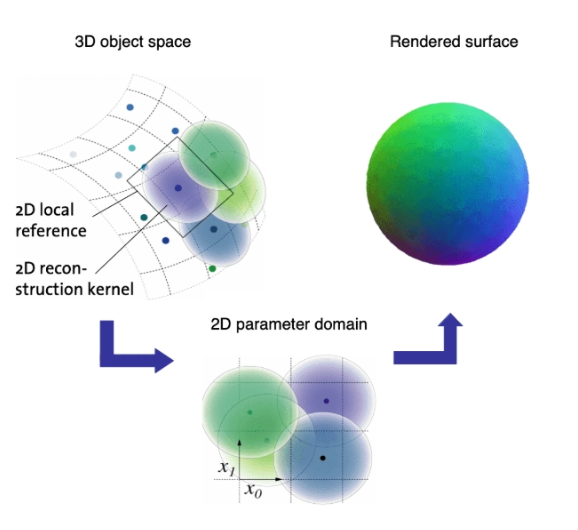
\includegraphics[width=0.5\textwidth]{images/surface_splatting.png}
    \caption{Surface splatting: each point is associated with a local surface element (surfel) that projects to an elliptical footprint.}
    \label{fig:surface_splatting}
\end{figure}

\paragraph{Volume splatting and EWA volume splatting.}
Volume splatting extends splatting to volumetric fields, closer to radiance-field rendering. In EWA volume splatting \cite{zwicker2002ewa}, volumetric primitives are often represented with Gaussian kernels. Gaussians are convenient because they are smooth, have easy derivatives for optimization, and admit convenient approximations under affine maps. In particular, a 3D Gaussian can be projected to a 2D footprint; intuitively, this can be interpreted as integrating a volumetric contribution along the viewing direction and representing its image-plane effect as an elliptical kernel.

The first stage of 3DGS estimates camera intrinsics and extrinsics and produces a sparse point cloud, typically using COLMAP \cite{schoenberger2016sfm,schoenberger2016mvs}. The objective is not to build a dense mesh, but to obtain a geometric prior suitable for initializing Gaussian means.

Let the sparse point cloud be
\[
\mathcal{P}=\{\mathbf{p}_i\}_{i=1}^{N},\qquad \mathbf{p}_i\in\mathbb{R}^3.
\]
A common initialization sets the Gaussian centers to SfM points,
\[
\boldsymbol{\mu}_i=\mathbf{p}_i.
\]
Camera poses are required at training time to project Gaussians into each training view and compare the rendered image to the observed image.

\subsubsection{Gaussian Parameterization}
Each primitive is parameterized by mean $\boldsymbol{\mu}_i$, covariance $\boldsymbol{\Sigma}_i$, opacity $o_i$, and view-dependent appearance coefficients (typically spherical harmonics).

\begin{figure}[H]
    \centering
    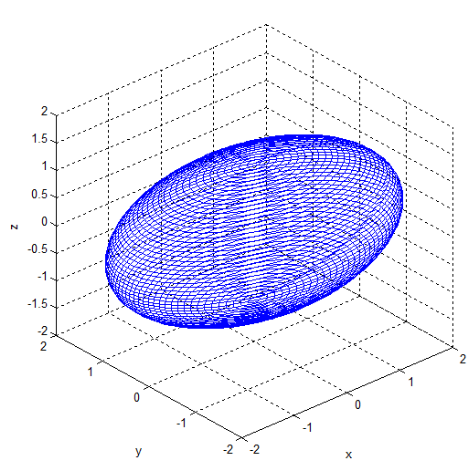
\includegraphics[width=0.35\textwidth]{images/3dGaussian.png}
    \caption{Single anisotropic 3D Gaussian primitive and its geometric parameters (center, covariance shape, and orientation).}
    \label{fig:gaussian_primitive_param}
\end{figure}

A typical Gaussian kernel is
\[
G_i(\mathbf{x})=\exp\!\left(-\frac{1}{2}(\mathbf{x}-\boldsymbol{\mu}_i)^\top
\boldsymbol{\Sigma}_i^{-1}(\mathbf{x}-\boldsymbol{\mu}_i)\right).
\]
To preserve valid covariance structure, $\boldsymbol{\Sigma}_i$ is parameterized through rotation and positive scales, e.g.
\[
\boldsymbol{\Sigma}_i=\mathbf{R}_i\mathbf{S}_i\mathbf{S}_i^\top\mathbf{R}_i^\top.
\]
In implementations, $\mathbf{R}_i$ is commonly represented by quaternions. Axis lengths are stored as \emph{log-scales} $\mathbf{s}_i\in\mathbb{R}^3$ and converted to $\boldsymbol{\sigma}_i=\exp(\mathbf{s}_i)$ before rasterization \cite{kerbl2023gaussian,tancik2023nerfstudio}: this enforces $\sigma>0$ without clipping under gradient descent and makes multiplicative shrink/grow steps more uniform when ellipsoid sizes span a wide range during densification.

The opacity $o_i$ modulates how strongly a Gaussian influences covered pixels. View-dependent color is represented by evaluating spherical harmonics as a function of viewing direction $\mathbf{d}$, denoted $\mathbf{c}_i(\mathbf{d})$.

\subsubsection{Splatting and rendering}
After initialization, rendering proceeds by splatting: each Gaussian is transformed to camera space, projected to the image plane, and rasterized as a 2D elliptical footprint. Unlike NeRF, 3DGS does not march rays through an implicit field; instead, it performs forward projection and accumulates contributions in image space.

At a high level, rendering executes the following steps:
\begin{enumerate}
    \item transform each Gaussian from world space to camera space;
    \item project the Gaussian center to the image plane;
    \item approximate the projected footprint as a 2D ellipse;
    \item evaluate the kernel response for pixels inside the footprint;
    \item composite contributions in depth order using alpha blending.
\end{enumerate}

\begin{figure}[H]
    \centering
    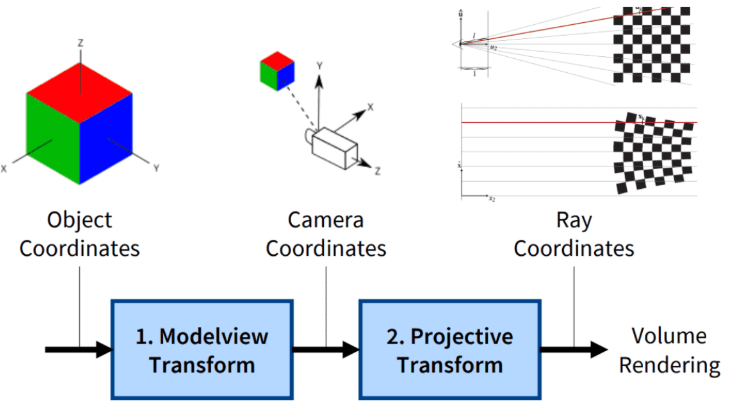
\includegraphics[width=0.5\textwidth]{images/complete_proiezioni.png}
    \caption{Multi-view projections involved in 3D Gaussian Splatting, relating camera observations to projected Gaussian structure.}
    \label{fig:multiview_projection_3dgs}
\end{figure}

\subsubsection{Transformation from world space to camera space}

Let $\boldsymbol{\mu} \in \mathbb{R}^3$ denote the Gaussian mean in world coordinates, with covariance $\boldsymbol{\Sigma} \in \mathbb{R}^{3 \times 3}$. Given the world-to-camera rotation $\mathbf{R}_{cw}$ and translation $\mathbf{t}_{cw}$, the mean in camera coordinates is

\[
\boldsymbol{\mu}_c = \mathbf{R}_{cw}\boldsymbol{\mu} + \mathbf{t}_{cw}.
\]

In homogeneous coordinates, this transformation can be written as

\[
\begin{bmatrix}
\boldsymbol{\mu}_c \\
1
\end{bmatrix}
=
\mathbf{T}_{cw}
\begin{bmatrix}
\boldsymbol{\mu} \\
1
\end{bmatrix},
\]

where $\mathbf{T}_{cw} \in \mathbb{R}^{4 \times 4}$ is the rigid transformation matrix.

The covariance transforms as

\[
\boldsymbol{\Sigma}_c = \mathbf{R}_{cw} \boldsymbol{\Sigma} \mathbf{R}_{cw}^\top,
\]

where the translation does not affect the covariance.

\subsubsection{Projection to ray space}

Following EWA volume splatting \cite{zwicker2002ewa}, \emph{ray space} is not the normalized image plane alone: it is a three-dimensional reparameterization of camera space in which the first two coordinates give the intersection of the viewing ray with the plane at unit depth ($z=1$), and the third records distance from the camera center along the ray. Let $\mathbf{x}_c=(x,y,z)^\top$ denote a point in camera coordinates (with $z>0$ in front of the camera). The mapping $g:\mathbb{R}^3\to\mathbb{R}^3$ is
\[
g(\mathbf{x}_c)=
\begin{pmatrix}
x/z \\[2pt]
y/z \\[2pt]
\|\mathbf{x}_c\|
\end{pmatrix},
\]
where $\|\mathbf{x}_c\|=\sqrt{x^2+y^2+z^2}$. The first two components coincide with \emph{normalized image coordinates} $(x/z,\,y/z)$; the third keeps a radial coordinate, so ray space remains $\mathbb{R}^3$ and should not be identified with image space $\mathbb{R}^2$.

The map $g$ is not affine. As in classical EWA splatting, one linearizes $g$ at the Gaussian mean $\boldsymbol{\mu}_c=(x,y,z)^\top$ using the Jacobian $\mathbf{J}\in\mathbb{R}^{3\times 3}$,
\[
\mathbf{J}=
\begin{pmatrix}
\frac{1}{z} & 0 & -\frac{x}{z^2} \\[4pt]
0 & \frac{1}{z} & -\frac{y}{z^2} \\[4pt]
\frac{x}{\|\mathbf{x}_c\|} & \frac{y}{\|\mathbf{x}_c\|} & \frac{z}{\|\mathbf{x}_c\|}
\end{pmatrix}_{\Big|\mathbf{x}_c=\boldsymbol{\mu}_c}.
\]
With $\boldsymbol{\Sigma}_c$ the camera-space covariance, a first-order propagated covariance in ray space is
\[
\boldsymbol{\Sigma}_{\mathrm{ray}} \approx \mathbf{J}\,\boldsymbol{\Sigma}_c\,\mathbf{J}^\top.
\]

\subsubsection{From ray space to the image-plane footprint}

Gaussians are closed under affine maps; under a fixed local linearization, the induced covariance remains quadratic in the tangent coordinates. The footprint used for splatting is a \emph{two-dimensional} Gaussian on the image plane (normalized coordinates). In the same local approximation, the marginal over the first two ray-space coordinates is obtained from the leading $2\times 2$ block of $\boldsymbol{\Sigma}_{\mathrm{ray}}$:
\[
\hat{\boldsymbol{\Sigma}} =
\begin{pmatrix}
[\boldsymbol{\Sigma}_{\mathrm{ray}}]_{11} & [\boldsymbol{\Sigma}_{\mathrm{ray}}]_{12} \\
[\boldsymbol{\Sigma}_{\mathrm{ray}}]_{21} & [\boldsymbol{\Sigma}_{\mathrm{ray}}]_{22}
\end{pmatrix},
\]
with mean in normalized coordinates $\boldsymbol{\mu}_{\mathrm{norm}}=(\mu_{c,1}/\mu_{c,3},\,\mu_{c,2}/\mu_{c,3})^\top$, i.e.\ the first two components of $g(\boldsymbol{\mu}_c)$. (Equivalently, one may motivate this reduction as integrating the 3D Gaussian contribution along the viewing direction in the EWA construction \cite{zwicker2002ewa}.)

\subsubsection{Projection to screen space}

Pixel coordinates apply the intrinsic matrix to homogeneous normalized coordinates. With
\[
\mathbf{K}=
\begin{pmatrix}
f_x & 0 & c_x \\
0 & f_y & c_y \\
0 & 0 & 1
\end{pmatrix},
\]
the projected mean is
\[
\boldsymbol{\mu}_{\mathrm{pix}}=
\begin{pmatrix}
f_x\,[\boldsymbol{\mu}_{\mathrm{norm}}]_1 + c_x \\
f_y\,[\boldsymbol{\mu}_{\mathrm{norm}}]_2 + c_y
\end{pmatrix}.
\]
For a diagonal scale from normalized to pixel coordinates (principal point handled in the mean), the screen-space covariance is
\[
\boldsymbol{\Sigma}_{\mathrm{pix}} \approx
\begin{pmatrix}
f_x & 0 \\
0 & f_y
\end{pmatrix}
\hat{\boldsymbol{\Sigma}}
\begin{pmatrix}
f_x & 0 \\
0 & f_y
\end{pmatrix}.
\]
Implementations often fold a single linearized map $\tilde{g}$ (normalized coordinates plus intrinsics in the first two components, distance in the third) and its $3\times 3$ Jacobian into one step before extracting the $2\times 2$ image block; the structure above matches that viewpoint while keeping the stages explicit.

The projected Gaussian footprint in screen space is
\[
g_i(\mathbf{x})=
\exp\!\left(
-\frac{1}{2}
(\mathbf{x}-\boldsymbol{\mu}_{\mathrm{pix},i})^\top
\boldsymbol{\Sigma}_{\mathrm{pix},i}^{-1}
(\mathbf{x}-\boldsymbol{\mu}_{\mathrm{pix},i})
\right),
\]
where $\mathbf{x}\in\mathbb{R}^2$ is a pixel coordinate.


\subsubsection{Rendering via Alpha Compositing}
At pixel $\mathbf{x}$, the opacity contribution of Gaussian $i$ combines learned opacity with the projected kernel:
\[
\alpha_i(\mathbf{x}) = o_i\,g_i(\mathbf{x}).
\]
Let Gaussians contributing to a pixel be sorted from front to back. The composited color is
\[
\mathbf{C}(\mathbf{x})=\sum_{i=1}^{N}T_i\,\alpha_i(\mathbf{x})\,\mathbf{c}_i(\mathbf{d}),\qquad
T_i=\prod_{j=1}^{i-1}\left(1-\alpha_j(\mathbf{x})\right),
\]
which mirrors alpha compositing used in volume rendering, but computed via rasterization of explicit primitives rather than ray integration through an MLP.

\begin{figure}[H]
    \centering
    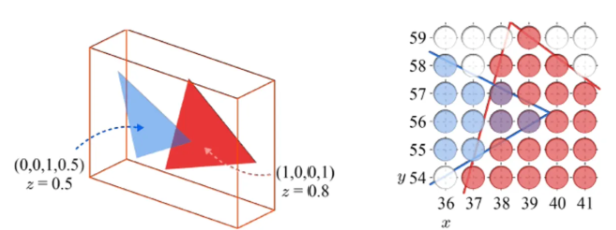
\includegraphics[width=0.5\textwidth]{images/alpha_blendig.png}
    \caption{Front-to-back alpha compositing intuition for accumulating Gaussian contributions along visibility order.}
    \label{fig:alpha_compositing_3dgs}
\end{figure}

\subsubsection{Photometric Optimization}
3DGS is trained with a photometric objective combining an $L_1$ term and a D-SSIM term:
\[
\mathcal{L}=(1-\lambda)\mathcal{L}_{1}+\lambda\mathcal{L}_{\text{D-SSIM}},
\qquad
\mathcal{L}_{\text{D-SSIM}}=\frac{1-\text{SSIM}(\hat{I},I)}{2},
\]
where $\hat{I}$ is the rendered image and $I$ is the ground truth for the sampled training view.

Let $\Theta=\{\boldsymbol{\mu}_i,\mathbf{s}_i,\mathbf{q}_i,o_i,\mathbf{c}_i\}_{i=1}^{N}$ denote all learnable parameters. Because rendering is differentiable, gradients $\nabla_\Theta \mathcal{L}$ can be computed and used in standard gradient-based optimizers:
\[
\Theta^{(t+1)}=\Theta^{(t)}-\eta \nabla_{\Theta}\mathcal{L}.
\]

\begin{algorithm}[htbp]
\caption{Optimization and Densification}
\label{alg:optimization_densification_3dgs}
\begin{algorithmic}[1]
\State \textbf{Input:} training image size $(w,h)$
\State $M \gets$ SfM points \Comment{initial Gaussian positions}
\State $S, C, A \gets \textsc{InitAttributes}()$ \Comment{covariances, colors, opacities}
\State $i \gets 0$
\While{not converged}
    \State $V, I_{\mathrm{gt}} \gets \textsc{SampleTrainingView}()$ \Comment{camera and image}
    \State $I \gets \textsc{Rasterize}(M,S,C,A,V)$ \Comment{see Algorithm~\ref{alg:rasterize_blending_3dgs}}
    \State $\mathcal{L} \gets \textsc{Loss}(I, I_{\mathrm{gt}})$
    \State $M,S,C,A \gets \textsc{AdamStep}(M,S,C,A,\nabla \mathcal{L})$
    \If{\textsc{IsRefinementIteration}($i$)}
        \For{all Gaussians $(\mu,\Sigma,c,\alpha)$}
            \If{$\alpha < \varepsilon$ \textbf{or} \textsc{TooLarge}($\mu,\Sigma$)}
                \State \textsc{RemoveGaussian}() \Comment{pruning}
            \EndIf
            \If{$\|\nabla_p \mathcal{L}\| > \tau_p$}
                \If{$\|\Sigma\| > \tau_s$}
                    \State \textsc{SplitGaussian}($\mu,\Sigma,c,\alpha$) \Comment{over-reconstruction}
                \Else
                    \State \textsc{CloneGaussian}($\mu,\Sigma,c,\alpha$) \Comment{under-reconstruction}
                \EndIf
            \EndIf
        \EndFor
    \EndIf
    \State $i \gets i + 1$
\EndWhile
\end{algorithmic}
\end{algorithm}

\subsubsection{Adaptive density control}
The initial SfM point cloud can be too sparse to represent fine details. 3DGS therefore modifies the set of primitives during training using \emph{adaptive density control}. Typical operations include:
\begin{itemize}
    \item \textbf{pruning} low-opacity or redundant Gaussians;
    \item \textbf{cloning} Gaussians in under-reconstructed regions;
    \item \textbf{splitting} large Gaussians into smaller ones when local detail is insufficient.
\end{itemize}
A common heuristic signal is the magnitude of the view-space positional gradient: large gradients often indicate that a Gaussian is important for explaining the image but is misaligned in position or scale.

\begin{figure}[H]
    \centering
    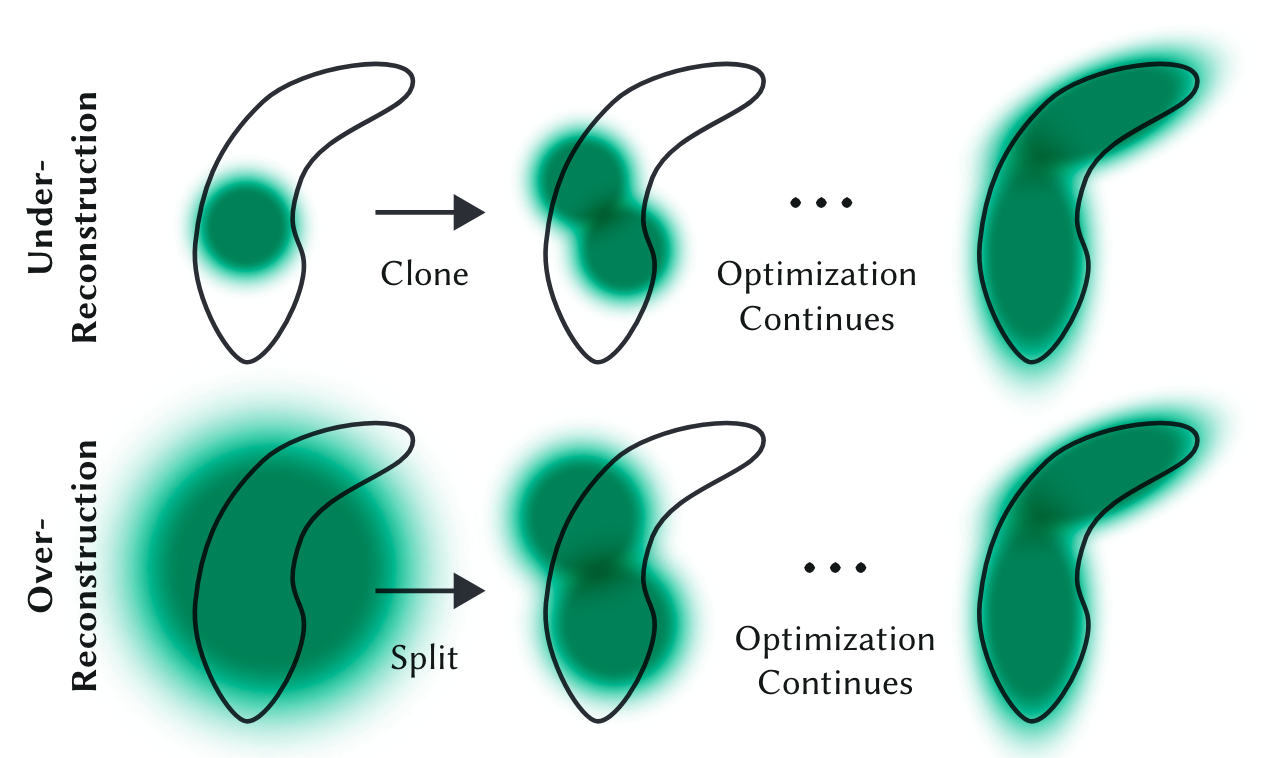
\includegraphics[width=0.5\textwidth]{images/adaptive_control_3Dgaussian.png}
    \caption{Adaptive density control in 3DGS (clone/split/prune) to improve coverage and local geometric detail.}
    \label{fig:3dgs_density_control}
\end{figure}

\subsubsection{Tile-based rasterization and visibility ordering}
Naively testing every Gaussian against every pixel is prohibitively expensive. Tile-based rasterization partitions the image into small tiles, assigns each Gaussian only to tiles intersected by its screen-space bounding box, sorts Gaussians by depth within each tile, and composites pixels using alpha blending.

\begin{figure}[H]
    \centering
    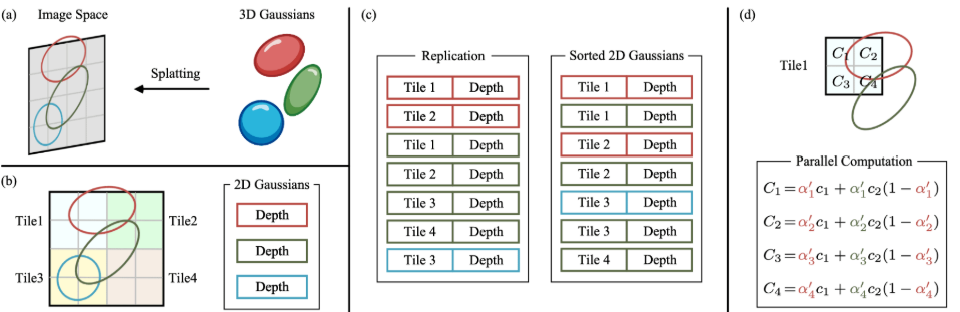
\includegraphics[width=0.7\textwidth]{images/complete_pipeline_3Dgaussian.png}
    \caption{3D Gaussian Splatting rendering flow: Gaussian parameterization, projection to screen-space ellipses, tile assignment, depth sorting, and compositing.}
    \label{fig:3dgs_projection_rasterization}
\end{figure}

\begin{algorithm}[htbp]
\caption{GPU Software Rasterization of 3D Gaussians}
\label{alg:rasterize_blending_3dgs}
\begin{algorithmic}[1]
\State \textbf{Input:} image size $(w,h)$, means $M$, covariances $S$, colors $C$, opacities $A$, view $V$
\State \textsc{CullGaussian}$(M,S,V)$ \Comment{frustum culling}
\State $M', S' \gets \textsc{ScreenspaceGaussians}(M,S,V)$ \Comment{transform}
\State $T \gets \textsc{CreateTiles}(w,h)$
\State $L,K \gets \textsc{DuplicateWithKeys}(M',T)$ \Comment{indices and keys}
\State \textsc{SortByKeys}$(K,L)$ \Comment{global sort}
\State $R \gets \textsc{IdentifyTileRanges}(T,K)$
\State $I \gets 0$ \Comment{initialize canvas}
\For{all tiles $t$ in $T$}
    \For{all pixels $i$ in $t$}
        \State $r \gets \textsc{GetTileRange}(R,t)$
        \State $I[i] \gets \textsc{BlendInOrder}(i,L,r,K,M',S',C,A)$
    \EndFor
\EndFor
\State \Return $I$
\end{algorithmic}
\end{algorithm}



\subsubsection{Limitations for Geometry Recovery}
Despite strong rendering quality, standard 3DGS still optimizes image consistency rather than explicit surface regularity. As a result, extracted geometry can be noisy, topologically ambiguous, or unstable in low-texture and occluded regions.

Moreover, thin structures and poorly observed regions can be represented by broad anisotropic blobs that explain color but do not correspond to physically plausible surfaces. This limitation motivates additional geometric supervision and structural priors, as developed in later chapters.

A practical manifestation of this behavior is the presence of \emph{floaters} (or floating Gaussians): small primitives that remain in incorrect 3D positions without matching a real surface (Figure~\ref{fig:floaters_example}). Training minimizes only the photometric loss $\mathcal{L}_{\mathrm{rgb}}$ (Section~2.3.5); for each Gaussian, position, scale, and opacity receive coupled gradients from that scalar objective through the rasterizer. If a misplaced primitive lowers $\mathcal{L}_{\mathrm{rgb}}$ on the training views where it is visible---for example by explaining residual color in poorly observed, reflective, or transparent regions---gradient descent has no incentive to remove it: its parameters sit at a \emph{local minimum} of $\mathcal{L}_{\mathrm{rgb}}$ (a stationary point of the loss landscape), meaning small joint changes to $(\boldsymbol{\mu},\mathbf{s},\alpha)$ would increase image error even though the 3D placement is wrong. Standard opacity-based pruning removes faint splats but does not penalize incorrect geometry directly; weak COLMAP initialization and subsequent densification can make such loss-minimizing yet geometrically invalid configurations more likely.

\begin{figure}[H]
    \centering
    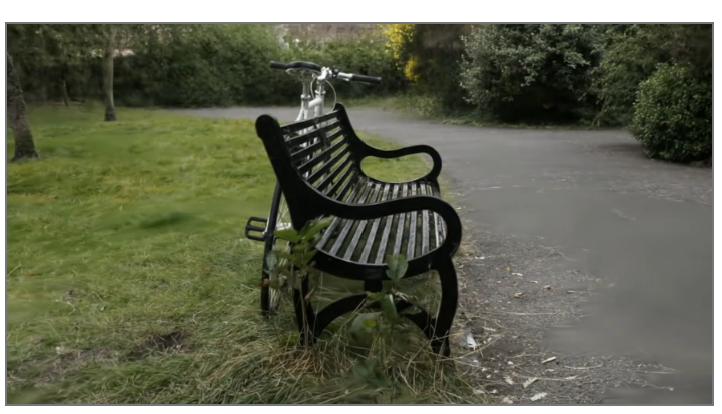
\includegraphics[width=0.35\textwidth]{images/floater_point.png}
    \caption{Example of floating Gaussians (floaters): primitives that reduce $\mathcal{L}_{\mathrm{rgb}}$ where they are seen but sit at geometrically invalid 3D locations.}
    \label{fig:floaters_example}
\end{figure}

\section{Depth in Neural Rendering}
To bridge appearance-driven rendering and geometry-aware optimization, this section focuses on the role of depth signals in neural rendering pipelines.

\subsection{Depth as Expected Value Along a Ray}
Neural radiance fields and many splatting-style renderers represent partially transparent media along viewing rays. As a consequence, a pixel does not correspond to a single surface intersection, but to an integral (or discrete sum) of contributions along the ray. Depth supervision must therefore specify \emph{which} notion of depth is being enforced.

\paragraph{Discrete volume rendering along a ray.}
Consider a camera ray through pixel $(x,y)$, with ordered samples indexed by $n=1,\dots,N$. Let $z_n$ denote the distance along the ray associated with sample $n$ (for example, the $z$ coordinate in camera space, or the Euclidean distance from the camera center, depending on implementation). Let $\alpha_n\in[0,1]$ denote the opacity (or occupancy) predicted at sample $n$, and let $T_n$ denote the transmittance up to sample $n$, i.e., the probability that the ray reaches sample $n$ without being fully stopped by earlier material.

Under the standard NeRF-style alpha compositing model, one defines
\[
T_1=1,\qquad
T_n=\prod_{k=1}^{n-1}(1-\alpha_k),\quad n>1,
\]
and the compositing weight for sample $n$ is $w_n=\alpha_n T_n$.

\paragraph{Accumulated depth vs.\ expected depth.}
With compositing weights defined, two common scalar summaries of ray depth are the \emph{accumulated depth} and the \emph{expected depth}. They can be written as
\begin{equation}
d_{x,y}^{\mathrm{acc}}=\sum_{n=1}^{N} z_n\,\alpha_n\,T_n,
\label{eq:depth_accumulated}
\end{equation}
and
\begin{equation}
d_{x,y}^{\mathrm{exp}}=
\frac{\sum_{n=1}^{N} z_n\,\alpha_n\,T_n}{\sum_{n=1}^{N} \alpha_n\,T_n}
=
\frac{d_{x,y}^{\mathrm{acc}}}{\sum_{n=1}^{N} w_n}.
\label{eq:depth_expected}
\end{equation}
Equation~\eqref{eq:depth_accumulated} aggregates depth contributions weighted by how much each sample affects the final pixel color. Equation~\eqref{eq:depth_expected} normalizes the same numerator by the total mass $\sum_n w_n$, producing a weighted average depth along the ray.

\paragraph{Relationship to compositing weights.}
From these definitions, and since $w_n=\alpha_n T_n$, the expected depth can equivalently be expressed as
\[
d_{x,y}^{\mathrm{exp}}=\sum_{n=1}^{N} \tilde{w}_n\, z_n,
\qquad
\tilde{w}_n=\frac{w_n}{\sum_{k=1}^{N} w_k},
\]
whenever $\sum_k w_k>0$. If $\sum_k w_k$ is substantially smaller than $1$, a large portion of the ray remains ``free space''; in that regime, depth summaries become sensitive to how ``empty space'' is handled numerically (epsilon stabilization, background models, or sky handling).

\paragraph{Semantic differences and failure modes.}
At this point it is useful to clarify interpretation: accumulated depth and expected depth answer different questions. The accumulated quantity grows with both geometry and visibility mass; the expected depth isolates a \emph{mean} depth under the induced distribution $\tilde{w}_n$. Both are fragile in qualitatively difficult cases:
\begin{itemize}
    \item \textbf{Multi-modality along a ray:} semi-transparent surfaces, foliage, fences, or motion blur can create multiple separated modes in $w_n$. Any single scalar depth collapses this structure and can be unstable under small changes in $\alpha_n$.
    \item \textbf{View dependence:} if opacity is view-dependent, depth summaries can change between cameras even for a fixed world point, which is problematic when enforcing multi-view consistency.
    \item \textbf{Scale alignment:} monocular depth priors are often defined up to unknown scale (and sometimes shift). Comparing $d^{\mathrm{exp}}$ to such priors therefore requires explicit alignment per image or per scene.
\end{itemize}

\subsection{Monocular Metric Depth Estimation}
To complement renderer-internal depth definitions, monocular depth estimation aims to predict a dense depth map from a single RGB image. In robotics and metrology, one often desires \emph{metric} depth in real-world units. However, many high-performing monocular models are trained to predict \emph{relative} depth up to an unknown affine ambiguity (scale and possibly shift), because diverse training domains do not share a single consistent metric scale.

\paragraph{From relative predictions to metric depth.}
In practical pipelines, metric depth is recovered by combining a relative-depth network with additional information, for example:
\begin{itemize}
    \item \textbf{Calibration and ground control:} known baselines, object sizes, or sparse LiDAR measurements to fix scale/shift.
    \item \textbf{Multi-view constraints:} epipolar geometry couples depths across views, which can reduce scale drift when cameras are calibrated.
    \item \textbf{Domain-specific fine-tuning:} supervised fine-tuning on datasets with metric ground truth (e.g., indoor RGB-D or automotive datasets).
\end{itemize}

\subsection{Depth Anything v3}
As a concrete model family aligned with these needs, Depth Anything 3 (DA3) is a general-purpose visual geometry model that predicts spatially consistent geometry from an arbitrary number of inputs (a single image, multi-view batches, or video), with or without known camera poses \cite{lin2025depthanything3}. The stated design goal is \emph{minimal modeling}: a plain pretrained vision transformer backbone (e.g., DINOv2) without bespoke geometric modules, trained to predict a compact set of dense outputs that still encode enough information to recover camera motion and scene structure.

\paragraph{Positioning relative to Depth Anything 1--2.}
Depth Anything (DA1) established a strong monocular foundation model by scaling dataset diversity and using large-scale training strategies that combine labeled and unlabeled data \cite{yang2024depth}. Depth Anything V2 (DA2) refined robustness and detail, producing monocular relative-depth models widely used as priors in 3D pipelines \cite{yang2024depthanythingv2}.

DA3 marks a generational shift in the series: it expands the operating regime from ``single image in, single depth map out'' to \emph{any-view} inference, jointly reasoning about multiple images and producing outputs that support consistent fusion into point clouds and downstream 3D representations \cite{lin2025depthanything3}. In monocular mode, DA3 is reported to surpass DA2 while preserving strong detail and robustness \cite{lin2025depthanything3}.

\paragraph{Core outputs: depth maps and ray maps.}
Given $N_v$ input images $\{\mathbf{I}_i\}_{i=1}^{N_v}$, DA3 produces per-view dense depth maps $\mathbf{D}_i$ aligned with pixels, and additionally predicts dense \emph{ray maps} that represent camera rays in a form that can be fused with depth to recover 3D points without directly regressing a rotation matrix with hard orthogonality constraints \cite{lin2025depthanything3}. Intuitively, predicting rays together with depths is a way to unify pose and geometry in a single feed-forward framework: depth explains ``how far along the ray'', while the ray field explains ``which ray belongs to each pixel in a global frame''.

\paragraph{Architecture (what is minimal and what is not).}
DA3 uses a ViT backbone and introduces an \emph{input-adaptive} cross-view self-attention mechanism implemented by reordering tokens in selected transformer blocks, enabling cross-image information exchange without changing the backbone architecture class \cite{lin2025depthanything3}. A dual DPT-style decoder head then predicts depth and ray maps from shared intermediate features, using separate fusion branches so the two tasks interact while avoiding redundant intermediate representations \cite{lin2025depthanything3}.

When camera intrinsics/extrinsics are known, DA3 can encode them as additional tokens that participate in attention; when unknown, a learnable camera token provides a consistent placeholder so the same model can operate in both posed and pose-free settings \cite{lin2025depthanything3}.

\begin{figure}[H]
    \centering
    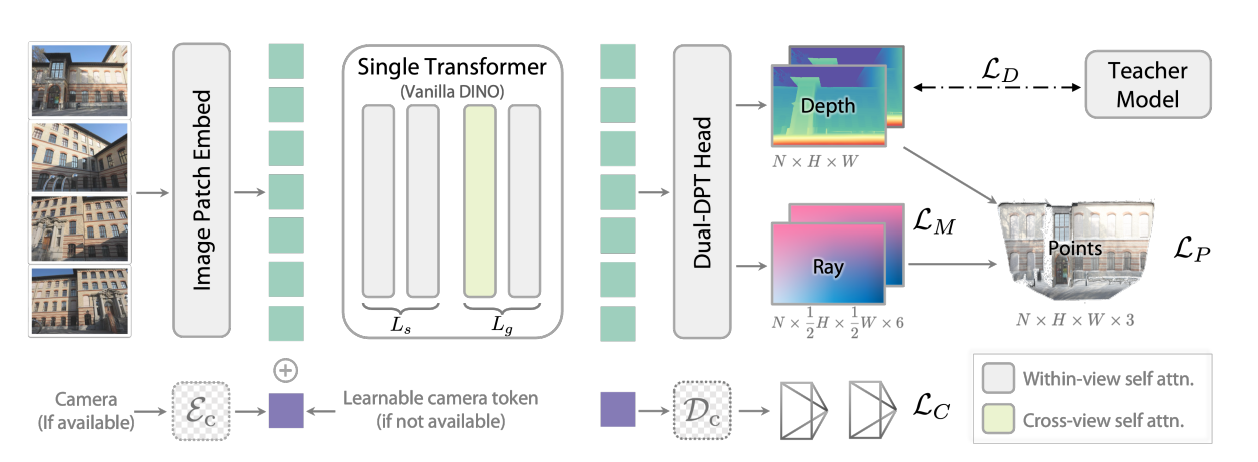
\includegraphics[width=0.8\textwidth]{images/pipelinedv3.png}
    \caption{Depth Anything 3 architecture (adapted from \cite{lin2025depthanything3}). $N$ input views are patch-embedded and processed by a DINO transformer with alternating within-view ($L_s$) and cross-view ($L_g$) self-attention. A dual-DPT head predicts per-view depth and ray maps; depth is supervised against a teacher model ($\mathcal{L}_D$), while ray maps and lifted 3D points are trained with $\mathcal{L}_M$ and $\mathcal{L}_P$. When camera parameters are unknown, a learnable camera token feeds an optional pose decoder ($\mathcal{L}_C$).}
    \label{fig:da3_pipeline}
\end{figure}

\paragraph{Training as teacher--student with pseudo-depth alignment (padre--figlio).}
DA3 is trained on heterogeneous supervision sources (synthetic renders, reconstructions, and real captures). Real-world depth supervision is often sparse, incomplete, or noisy; training directly on such labels can limit fine detail \cite{lin2025depthanything3}. DA3 therefore adopts a teacher--student paradigm closely inspired by prior Depth Anything pseudo-labeling ideas \cite{yang2024depth,yang2024depthanythingv2}:
\begin{itemize}
    \item \textbf{Teacher (padre):} a strong monocular relative-depth model trained on large synthetic data to produce dense pseudo-depth with high-frequency detail.
    \item \textbf{Student (figlio):} the DA3 model trained to match pseudo labels while remaining anchored to original sparse/noisy ground truth.
\end{itemize}
Crucially, the teacher pseudo-depth is aligned to the available real measurements using robust scale/shift fitting (the paper specifies RANSAC least squares), intended to preserve global geometric fidelity while gaining dense completeness \cite{lin2025depthanything3}. The DA3 teacher extends DA2-style training along two axes emphasized in the paper: \emph{data scaling} on a substantially expanded synthetic corpus, and a revised \emph{depth representation} (predicting scale--shift invariant depth rather than disparity, and using an exponential parameterization of depth to improve near-range sensitivity) \cite{yang2024depthanythingv2,lin2025depthanything3}; its objective combines multiple geometric signals (including gradient supervision and additional normal-based terms described in the paper) to improve local planarity and edge behavior for downstream 3D use \cite{lin2025depthanything3}. The student is trained with a composite objective that supervises predicted depth and ray maps, encourages predicted point maps to agree with supervision, includes an optional camera prediction term when poses are used, and uses a depth-gradient loss to preserve sharp discontinuities while maintaining smooth planar regions \cite{lin2025depthanything3}. The paper also describes a training schedule where supervision transitions from ground-truth signals to teacher pseudo-labels during training, which operationalizes the idea that early training should respect metric/sparse constraints, while later training can safely densify detail \cite{lin2025depthanything3}.

\paragraph{Implementation-scale training details (why DA3 is not ``just a bigger DA2'').}
The paper reports large-scale training on many public datasets spanning synthetic, LiDAR, and reconstruction-derived labels, with a long schedule on modern accelerators and a deliberately chosen base resolution grid designed to be compatible with common aspect ratios \cite{lin2025depthanything3}. Beyond dataset scale, two training mechanisms are particularly important for thesis readers:
\begin{itemize}
    \item \textbf{Curriculum from clean constraints to dense pseudo labels:} switching supervision sources during training reduces the risk that dense-but-imperfect pseudo depth overwhelms early optimization before the model has learned coarse geometric consistency \cite{lin2025depthanything3}.
    \item \textbf{Randomized pose conditioning:} occasionally providing ground-truth intrinsics/extrinsics during training teaches the model to exploit pose cues when available, while still remaining usable when poses are unknown at inference time \cite{lin2025depthanything3}.
\end{itemize}



\paragraph{Use in this thesis.}
In the Splatfacto implementation developed for this thesis, DA3 is used only as a \emph{monocular} depth prior: for each training view, a dense depth target is computed independently from the ground-truth RGB image. The checkpoint \textbf{DA3METRIC-LARGE} (\emph{Monocular Metric Depth}) is used rather than a relative-depth variant; its output is converted to metric depth in meters using the known focal length in pixels, so no per-image affine scale--shift alignment is required when supervising rendered depth in camera space. Poses and intrinsics are taken from COLMAP, not from DA3; the multi-view cross-attention, ray maps, and optional camera head of the full DA3 framework are outside the scope of this work.



\section{Surface-Based Representations}
After depth priors, the discussion shifts to explicit parametric geometry used in this thesis to improve structural control.

\subsection{B\'ezier Curves and Surfaces}
This section reviews B\'ezier curves and tensor-product B\'ezier surfaces as explicit parametric geometry. The definitions below underpin the surface-based modifications developed in Chapter~\ref{chap:methodology}: B\'ezier models offer a compact set of control parameters that induce smooth geometry and support stable optimization under image-based supervision.

\paragraph{Bernstein basis and B\'ezier curves.}
A degree-$M$ B\'ezier curve is a polynomial curve in $\mathbb{R}^d$ parameterized by $t\in[0,1]$:
\[
\mathbf{B}(t)=\sum_{j=0}^{M} B_j^{M}(t)\,\mathbf{p}_j,
\qquad
B_j^{M}(t)=\binom{M}{j}(1-t)^{M-j}t^{j},
\]
where $\{\mathbf{p}_j\}_{j=0}^{M}$ are control points. The basis functions $B_j^{M}$ are nonnegative on $[0,1]$ and partition unity, $\sum_j B_j^{M}(t)=1$. Consequently, $\mathbf{B}(t)$ lies in the convex hull of the control polygon for all $t\in[0,1]$ (convex-hull property), which is useful as a geometric prior: feasible shapes are globally constrained by a small number of control points.

\begin{figure}[H]
    \centering
    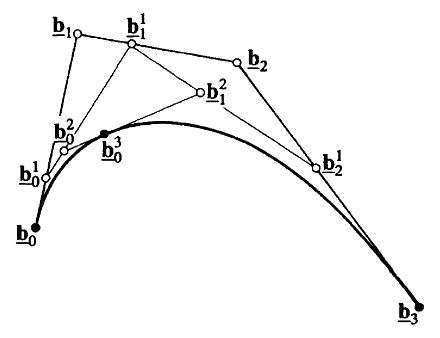
\includegraphics[width=0.5\textwidth]{images/curve_di_bezier.png}
    \caption{B\'ezier curve example with control polygon and resulting smooth trajectory, illustrating Bernstein interpolation and convex-hull behavior.}
    \label{fig:bezier_curve_example}
\end{figure}

\paragraph{Geometric meaning of control points.}
From this basis representation, the geometric role of control points becomes clearer. Increasing the degree increases expressivity at the cost of more parameters and potential oscillation (Runge-type phenomena) if control points are poorly placed. In practice, complex shapes are represented by joining multiple B\'ezier segments with continuity constraints at junctions. B\'ezier curves are differentiable polynomials; the tangent direction follows from differentiating the Bernstein expansion. For optimization, this matters because objective functions that depend on positions on the curve (e.g., through rendering) can backpropagate gradients to control points through the chain rule, provided downstream operations are differentiable.

\paragraph{Tensor-product B\'ezier surfaces.}
Extending the same idea from curves to surfaces, a tensor-product B\'ezier patch maps parameters $(u,v)\in[0,1]^2$ into $\mathbb{R}^3$ by separating variation along $u$ and $v$:
\[
\mathbf{S}(u,v)=\sum_{i=0}^{M_u}\sum_{j=0}^{M_v}
B_i^{M_u}(u)\,B_j^{M_v}(v)\,\mathbf{p}_{i,j},
\]
where $\{\mathbf{p}_{i,j}\}$ form a rectangular control net. Intuitively, each iso-$v$ curve is a B\'ezier curve in $u$, and each iso-$u$ curve is a B\'ezier curve in $v$. This separability is convenient for sampling, texturing, and enforcing regularity: smoothness in $u$ and $v$ is inherited from the smoothness of Bernstein polynomials.

\begin{figure}[H]
    \centering
    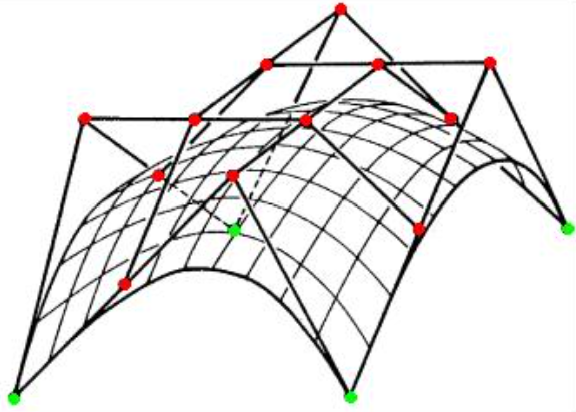
\includegraphics[width=0.5\textwidth]{images/surface_bezier.png}
    \caption{Tensor-product B\'ezier surface with control net: variation along $(u,v)$ generates a smooth parametric patch in $\mathbb{R}^3$.}
    \label{fig:bezier_surface_example}
\end{figure}

\paragraph{Local shape control and continuity across patches.}
Moving one control point $\mathbf{p}_{i,j}$ influences the surface locally, with influence strongest near the corresponding parameter region but generally nonzero across the patch (global support of Bernstein basis on $[0,1]^2$). Complex objects are therefore often modeled by multiple patches with $C^0$, $C^1$, or higher continuity enforced along shared boundaries by constraining control nets (e.g., colinearity of adjacent control edges for $C^1$ transitions).

\subsection{B\'ezier-Based Splatting Approaches}
To connect these geometric primitives with rendering practice, recent work on \emph{B\'ezier Splatting} studies how to combine parametric B\'ezier primitives with Gaussian splatting-style rasterization for differentiable vector graphics \cite{liu2025bezier}. The central theoretical idea is to replace exact boundary-centric rasterization of curves (as in classical differentiable vector renderers) with an explicit, kernel-based accumulation of Gaussians placed along, and in the vicinity of, B\'ezier curves, exploiting the fact that Gaussian footprints yield stable spatial gradients in image space while remaining compatible with fast tile-based rasterization \cite{liu2025bezier,kerbl2023gaussian}.

\paragraph{From curves in 2D to surfaces in 3D (conceptual lift).}
In vector graphics, B\'ezier curves live in $\mathbb{R}^2$ and partition the image into stroke and non-stroke regions. In 3D scene reconstruction, one may analogously treat a B\'ezier \emph{surface} $\mathbf{S}(u,v)\subset\mathbb{R}^3$ as a low-dimensional geometric scaffold that explains a subset of the scene (typically an object-centric region). The same structural principle applies:
\begin{itemize}
    \item \textbf{Explicit parameterization:} geometry is controlled by a control net rather than by unconstrained point clouds.
    \item \textbf{Differentiable sampling:} points $\mathbf{S}(u,v)$ (and local frames induced by partial derivatives $\partial_u \mathbf{S}$, $\partial_v \mathbf{S}$) can be used as anchors for volumetric primitives.
    \item \textbf{Splatting viewpoint:} rendering can be understood as projecting localized kernels to the image plane and compositing contributions, rather than solving hard boundary predicates per pixel.
\end{itemize}

\paragraph{How this thesis uses surfaces ``like curves'' at a high level.}
At the level of theory (not implementation), the methodological analogy is:
\begin{enumerate}
    \item define an explicit B\'ezier \emph{surface patch} that approximates visible object geometry in 3D;
    \item generate a structured set of 3D locations on (and optionally near) the patch by sampling $(u,v)$ and optional offsets along a local normal direction;
    \item associate each location with a localized volumetric primitive whose parameters are tied to the patch (positionally anchored, with anisotropy aligned to local tangents);
    \item optimize patch parameters jointly with the rendering objective, so image residuals update the control net through the sampled primitive chain.
\end{enumerate}
This mirrors the 2D B\'ezier splatting philosophy, ``optimize parametric geometry through splatted kernels'', while replacing curve arclength by surface parameters $(u,v)$ and replacing planar strokes by embedded surfaces in $\mathbb{R}^3$ \cite{liu2025bezier}.

\paragraph{Pruning/densification as a geometric analogue.}
B\'ezier Splatting emphasizes adaptive allocation of curve capacity: remove negligible primitives and densify where reconstruction error remains high, interpreting densification as enlarging the effective receptive field of the parametric model \cite{liu2025bezier}. The same conceptual mechanism carries over to surfaces: patch refinement can be viewed as reallocating representational budget where photometric gradients indicate persistent mismatch between rendered and observed images.

\section{Semantic Object Segmentation}
To support object-centric initialization, many 3D reconstruction pipelines need to isolate a subset of geometry and appearance that corresponds to a user-specified entity. In this thesis, semantic isolation is obtained by combining \emph{text-conditioned localization} with \emph{promptable segmentation}:
\begin{itemize}
    \item Grounding DINO proposes boxes (and associated language alignments) from free-form text \cite{liu2023groundingdino}.
    \item SAM~2 turns boxes/clicks/masks into high-quality region masks and can propagate them across views or time \cite{ravi2024sam2}.
\end{itemize}
The following subsections summarize the underlying models at the same level of technical depth used for depth foundation models elsewhere in this chapter.

\subsection{GroundingDINO}
In multi-view pipelines, text prompts can be applied independently per image (or on a reference view) to obtain candidate boxes. These boxes define image regions whose corresponding rays and sparse points can be aggregated into an object-centric working set. Grounding DINO is an open-set object detector that accepts a free-text prompt and predicts a set of bounding boxes aligned with noun phrases in the text \cite{liu2023groundingdino}. The motivating problem is \emph{open-set} (or open-vocabulary) detection: the model must generalize beyond a fixed category list by grounding visual regions in language, rather than classifying into a closed label space \cite{liu2023groundingdino}.

\paragraph{From closed-set detection to language-grounded detection.}
Classical detectors map each region embedding to one of $K$ training categories. Open-set detectors instead seek a joint embedding space where a region can be matched to arbitrary text tokens (words or phrases). Grounding DINO follows the GLIP-style perspective that object detection can be formulated as phrase grounding at scale, but requires language to be fused throughout the pipeline rather than at a single stage \cite{liu2023groundingdino}. Fusion is structured in three phases: (A) feature enhancement in the neck, (B) query initialization, and (C) decoding and refinement in the head. Earlier open-set systems often integrated text in only one phase; Grounding DINO applies cross-modal fusion in all three to improve alignment between visual features and the prompt \cite{liu2023groundingdino}.

\paragraph{Architecture overview.}
Grounding DINO is a dual-encoder, single-decoder architecture \cite{liu2023groundingdino}:
\begin{enumerate}
    \item \textbf{Image backbone:} extracts multi-scale image tokens (e.g., Swin-style hierarchical features).
    \item \textbf{Text backbone:} extracts token-level language embeddings (e.g., BERT-style contextualized tokens).
    \item \textbf{Feature enhancer (phase A):} performs cross-modal fusion by stacking self-attention and cross-attention blocks, including both text-to-image and image-to-text cross-attention, so that early visual features are already language-aware \cite{liu2023groundingdino}.
    \item \textbf{Language-guided query selection (phase B):} selects a fixed number of decoder queries from image tokens based on their compatibility with the text prompt.
    \item \textbf{Cross-modality decoder (phase C):} refines queries with additional image and text cross-attention layers before predicting boxes and aligned phrases \cite{liu2023groundingdino}.
\end{enumerate}

\begin{figure}[H]
    \centering
    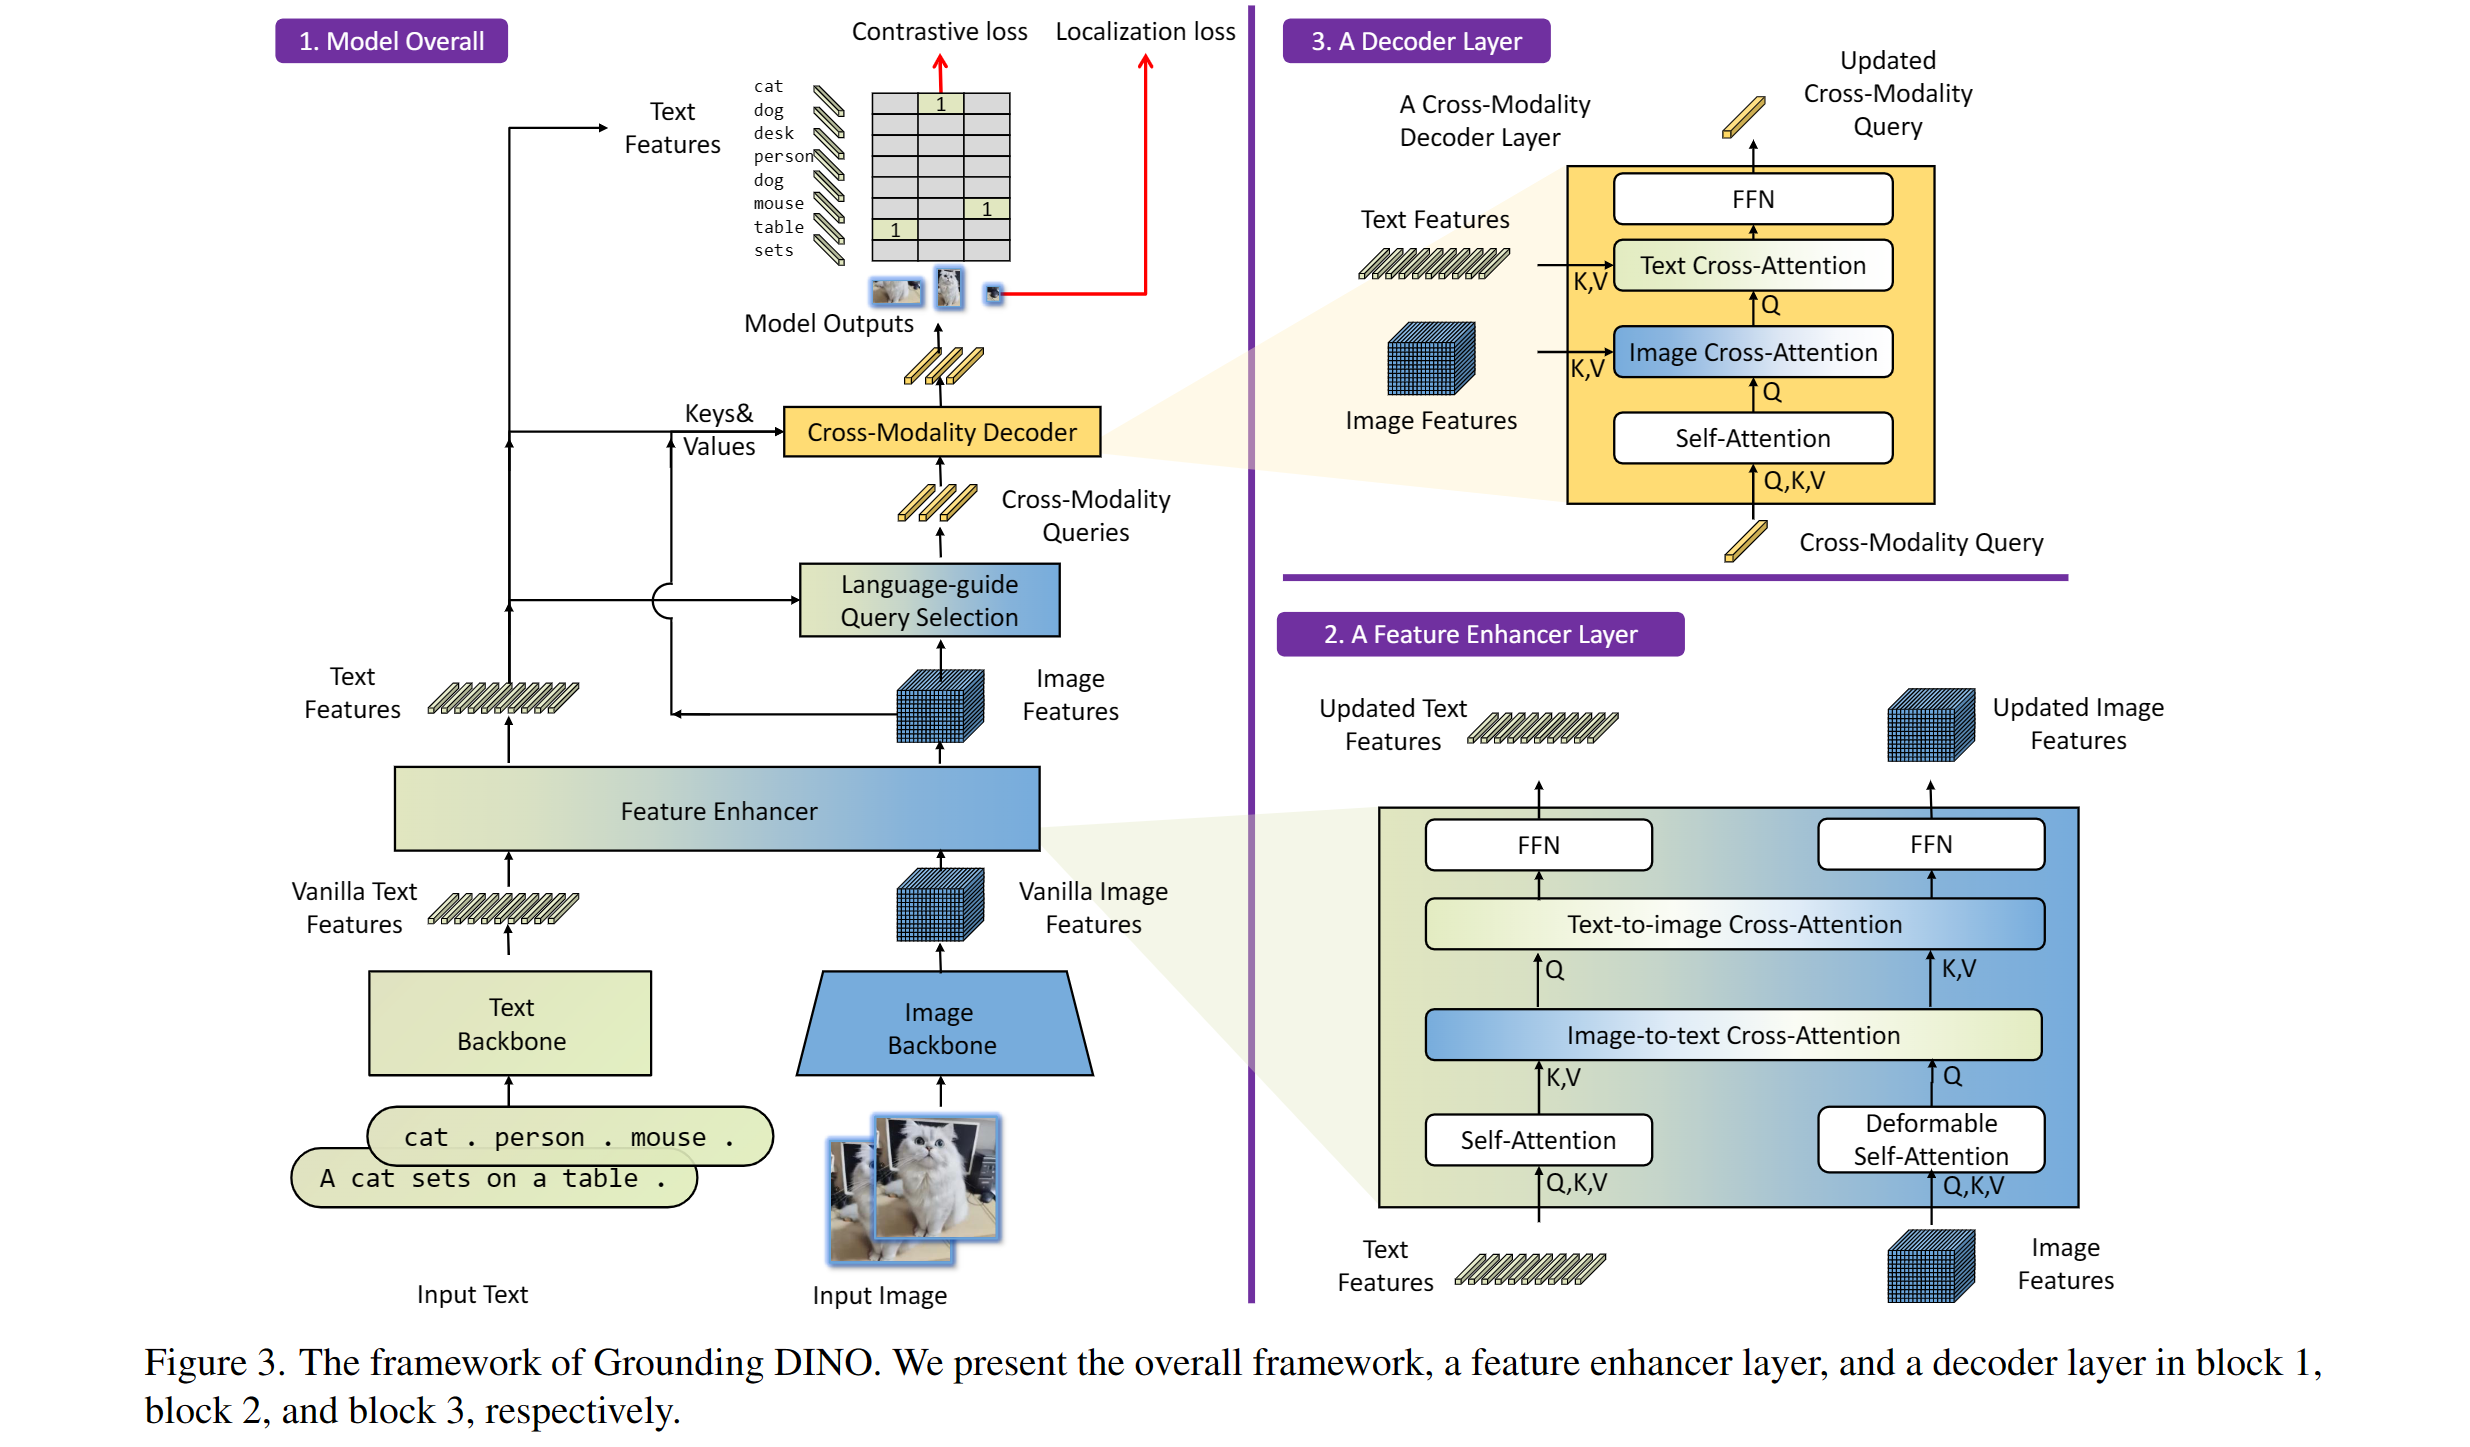
\includegraphics[width=0.8\textwidth]{images/groundingDino.png}
    \caption{Grounding DINO architecture overview with image/text encoders, cross-modal fusion, and language-guided detection outputs.}
    \label{fig:grounding_dino_architecture_overview}
\end{figure}

\paragraph{Language-guided query selection (mathematical intuition).}
Let image tokens be $\mathbf{X}_I\in\mathbb{R}^{N_I\times d}$ and text tokens be $\mathbf{X}_T\in\mathbb{R}^{N_T\times d}$. Grounding DINO selects $N_q$ image indices (typically $N_q=900$) by scoring each image token against the entire text sequence and taking top-$N_q$ locations:
\[
\mathcal{I}_{N_q}=\mathrm{Top}_{N_q}\!\left(\max_{j}(\mathbf{X}_I\mathbf{X}_T^\top)_{:,j}\right).
\]
Intuitively, this implements a soft ``visual saliency under the text prompt'': tokens that strongly align with any word/phrase in the prompt become initialization carriers for object queries \cite{liu2023groundingdino}. The selected indices are then combined with mixed query selection as in DINO: positional components are tied to encoder-derived anchors, while content components remain learnable \cite{liu2023groundingdino}.

\paragraph{Cross-modality decoder.}
Each decoder layer performs self-attention among queries, then updates queries with image cross-attention and an additional text cross-attention pathway. This design repeatedly injects textual constraints during box refinement, rather than conditioning only once \cite{liu2023groundingdino}.

\paragraph{Sub-sentence text representation.}
When prompts concatenate multiple category names, sentence-level encoding can lose token granularity, while naive word-level encoding can introduce spurious dependencies between unrelated words. Grounding DINO introduces a \emph{sub-sentence} representation with attention masks that block interactions between unrelated categories while preserving per-token features \cite{liu2023groundingdino}.


\paragraph{Training objective and matching.}
Grounding DINO follows DETR-style bipartite matching: predicted boxes are matched to ground-truth boxes, and losses are computed on matched pairs. Box regression uses $\ell_1$ and GIoU terms, while classification is treated as a contrastive problem between queries and text tokens with a focal loss on token logits \cite{liu2023groundingdino}. Auxiliary losses after encoder and intermediate decoder layers stabilize deep transformer training \cite{liu2023groundingdino}. The model is pre-trained on heterogeneous detection, grounding, and caption-style data with large-scale grounded supervision, which supports zero-shot transfer on benchmarks such as COCO, LVIS, ODinW, and referring-expression tasks \cite{liu2023groundingdino}. In this thesis, a short text prompt (e.g.\ ``wooden chair'' or ``laptop screen'') is sufficient to obtain candidate boxes on each view without scene-specific fine-tuning.

\subsection{SAM2}
SAM~2 is a foundation model for \emph{promptable visual segmentation} (PVS) that unifies interactive segmentation in images and videos \cite{ravi2024sam2}. A video is treated as a sequence of frames; an image is the special case of a one-frame sequence \cite{ravi2024sam2}.

\paragraph{Task definition: from SAM (image) to masklets (video).}
The PVS task accepts prompts on any frame, points, boxes, or masks, and produces a spatio-temporal mask (\emph{masklet}) for the target entity across frames \cite{ravi2024sam2}. This generalizes interactive video object segmentation: users can correct errors on later frames without restarting from scratch, because the model retains memory of prior prompts and predictions \cite{ravi2024sam2}.


\paragraph{Architecture.}
SAM~2 processes frames in a streaming fashion, consuming one frame at a time \cite{ravi2024sam2}. The main components are the following.

\textbf{Image encoder.} An MAE-pretrained hierarchical Hiera backbone runs once per frame and produces unconditioned, multi-scale spatial feature tokens \cite{ravi2024sam2}. High-resolution skip connections from the encoder bypass memory attention and feed directly into the mask decoder to preserve fine boundary detail.

\textbf{Memory attention.} A stack of $L$ transformer blocks conditions the current-frame tokens on a memory bank. Each block applies self-attention over the current-frame tokens, then cross-attention to stored spatial memories and to lightweight \emph{object pointer} vectors, followed by an MLP \cite{ravi2024sam2}. Vanilla attention is used throughout, enabling compatibility with efficient attention kernels.

\textbf{Prompt encoder and mask decoder.} The prompt encoder is identical to SAM's: sparse inputs (clicks, boxes) are represented as positional encodings summed with learned per-type embeddings, while mask prompts are embedded via convolutions. The decoder uses stacked two-way transformer blocks that jointly update prompt tokens and frame embeddings, and predicts multiple candidate masks under ambiguous prompts; the mask with highest predicted IoU is propagated when no corrective prompt resolves ambiguity \cite{ravi2024sam2}. A dedicated binary head predicts whether the target object is visible on the current frame, handling occlusion transparently.

\textbf{Memory encoder and memory bank.} After decoding, the memory encoder compresses the predicted mask by downsampling it with a convolutional module and adding it element-wise to the unconditioned frame embedding, followed by lightweight convolutional fusion layers \cite{ravi2024sam2}. The resulting spatial feature map is stored in a FIFO queue of up to $N$ recent frames; prompted frames are stored in a separate FIFO queue of up to $M$ slots. Temporal position encodings are added only to the $N$ recent-frame memories (to represent short-term motion), not to prompted-frame memories, because prompted frames may be temporally irregular at inference \cite{ravi2024sam2}.

\begin{figure}[H]
    \centering
    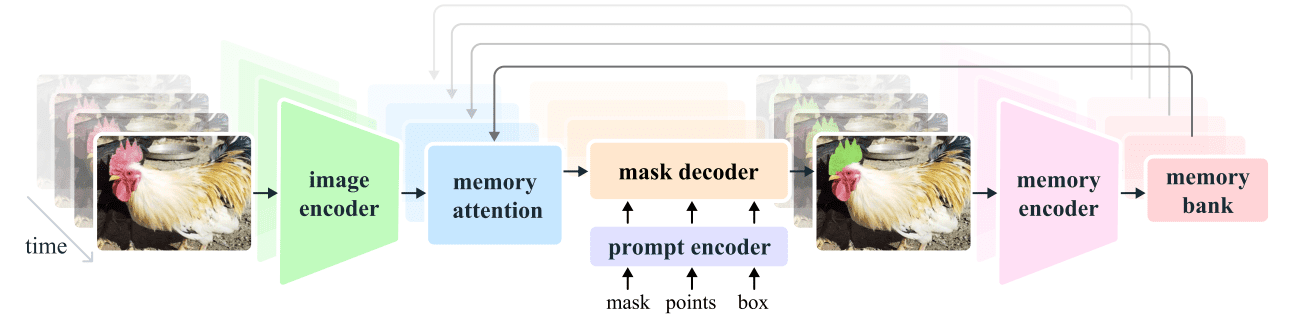
\includegraphics[width=0.95\textwidth]{images/sam2-architecture.png}
    \caption{SAM~2 streaming architecture with memory bank and memory attention for promptable segmentation across frames.}
    \label{fig:sam2_memory_bank_attention}
\end{figure}

\paragraph{Training and data.}
SAM~2 is trained jointly on images and short video clips by simulating interactive prompting: the model receives progressively richer prompts (mask, click, or box with prescribed probabilities) and is trained to sequentially predict ground-truth masklets, including corrective clicks sampled from disagreement regions \cite{ravi2024sam2}. Training is supported by a model-in-the-loop annotation engine that scales collection of diverse masklets, producing the SA-V dataset at a scale substantially larger than prior video segmentation datasets \cite{ravi2024sam2}.

\paragraph{Use in this thesis.}
In the implementation described in Chapter~\ref{chap:methodology}, SAM~2 is invoked through \texttt{SAM2ImagePredictor}: each training image is processed independently, prompted with the bounding box produced by Grounding DINO for that view. The temporal memory bank, which SAM~2 uses for video propagation, is therefore not activated. SAM~2 is used here purely for its strong single-image segmentation quality, which inherits from training on large and diverse data while remaining compatible with the unordered multi-view image collections produced by COLMAP.

